\subsection*{RQ1: scenarios and learning contexts}

The main research areas seems to be connected to schools and governance (Fig. \ref{fig:scenarios}).
This is confirmed by the fact that the target population of the studies and/or the community affected by the learning process is often the students.

Several publications present this scenario where students are involved in the development of an architectural or urban planning project in the city\cite{seitamaa-hakkarainen_architecture_2012}\cite{ulrich_lets_2013}\cite{beckett_augmented_2005}.

\begin{figure}[htb]
\centering
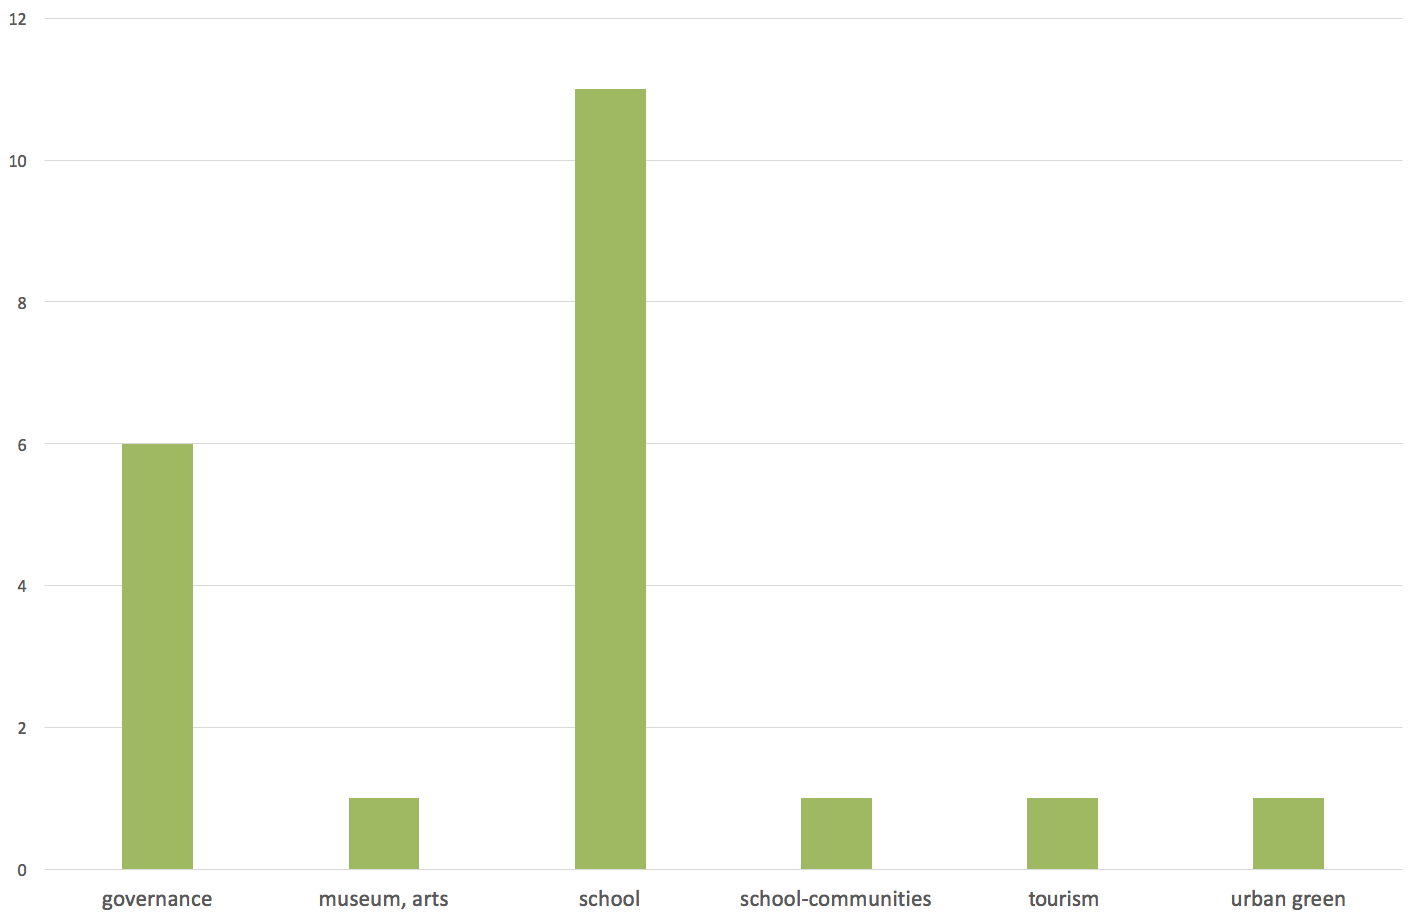
\includegraphics[width=12cm]{img/scenario}
\caption{Identified research scenarios.}
\label{fig:scenarios}
\end{figure}

This result can be correlated to the finding that more than 68\% of the articles present the concept of the city as a place where learning happens. This point of view is quite distinct to the more engaging concept of actively living the city learning behaviours and generating knowledge, which can be considered a lifelong learning experience to improve the quality of urban living.
As an example of this concept, some articles focus on promoting and teaching environmental-friendly practices like reducing the carbon footprint\cite{evans_give_2014} or reduce dependence on owned cars to satisfy mobility needs\cite{valle_cloud_2011}.


\subsection*{RQ2: publication pattern}

Research on smart-city learning gained approval and popularity quite constantly during the years. A relatively important amount of articles dates back to 2005, starting year of the chosen interval.

From 2006 a general increase in publications can be noted till 2014. The year 2015 was excluded from this statistic since not all research on the topic was yet published when articles were collected.

\begin{figure}[htb]
\centering
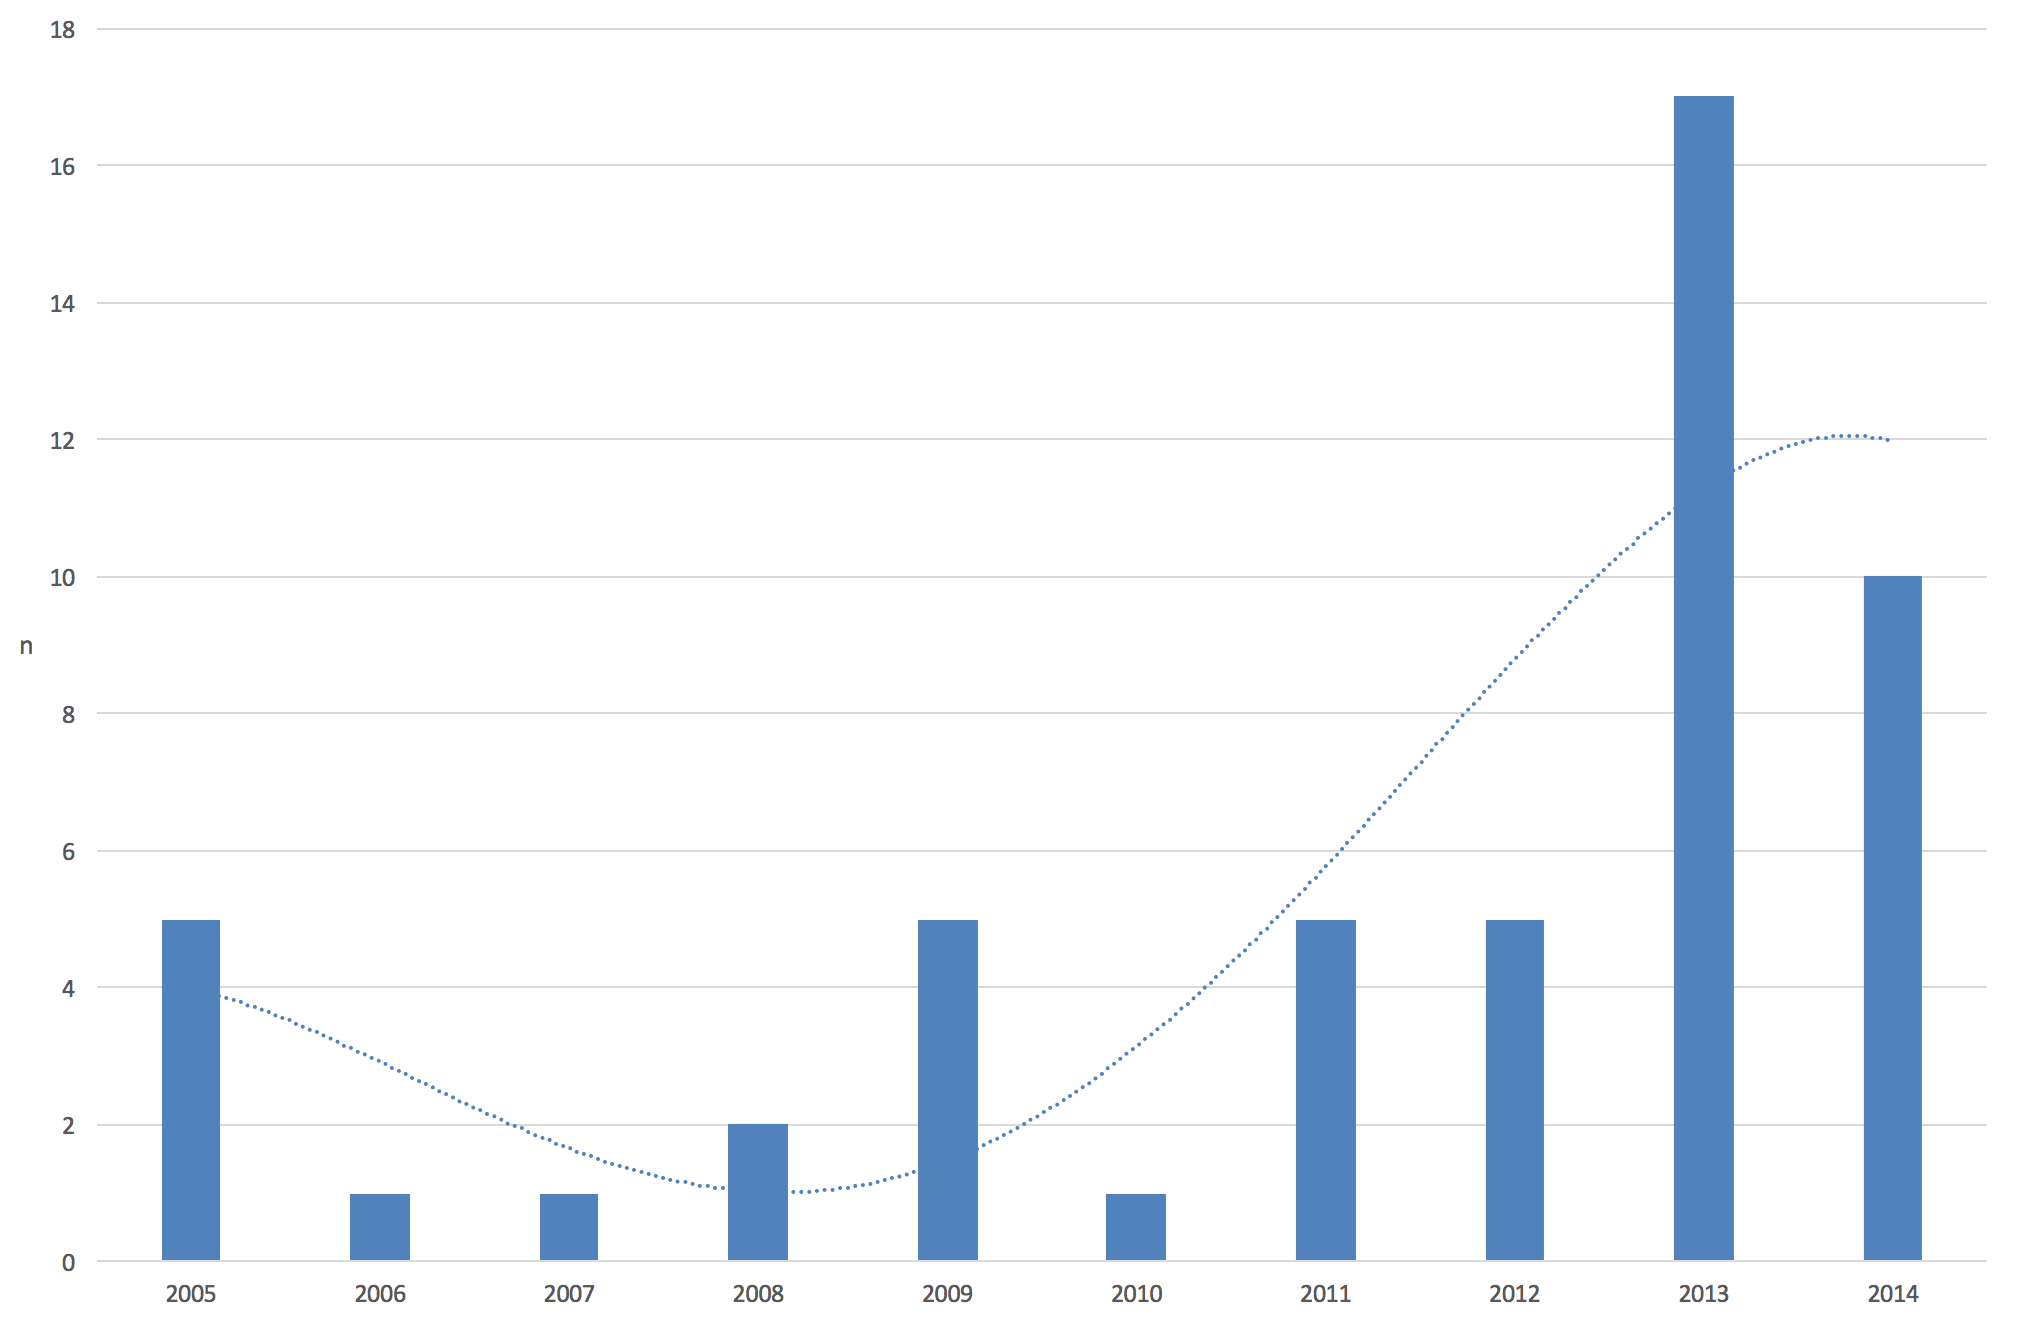
\includegraphics[width=12cm]{img/years}
\caption{Research publications per year.}
\label{fig:years}
\end{figure}

Selected articles are almost equally divided between international conference proceeding publications and journal or book chapters.
Publications from international journals remain the overall prevalent group.

% \begin{figure}[htb]
% \centering
% 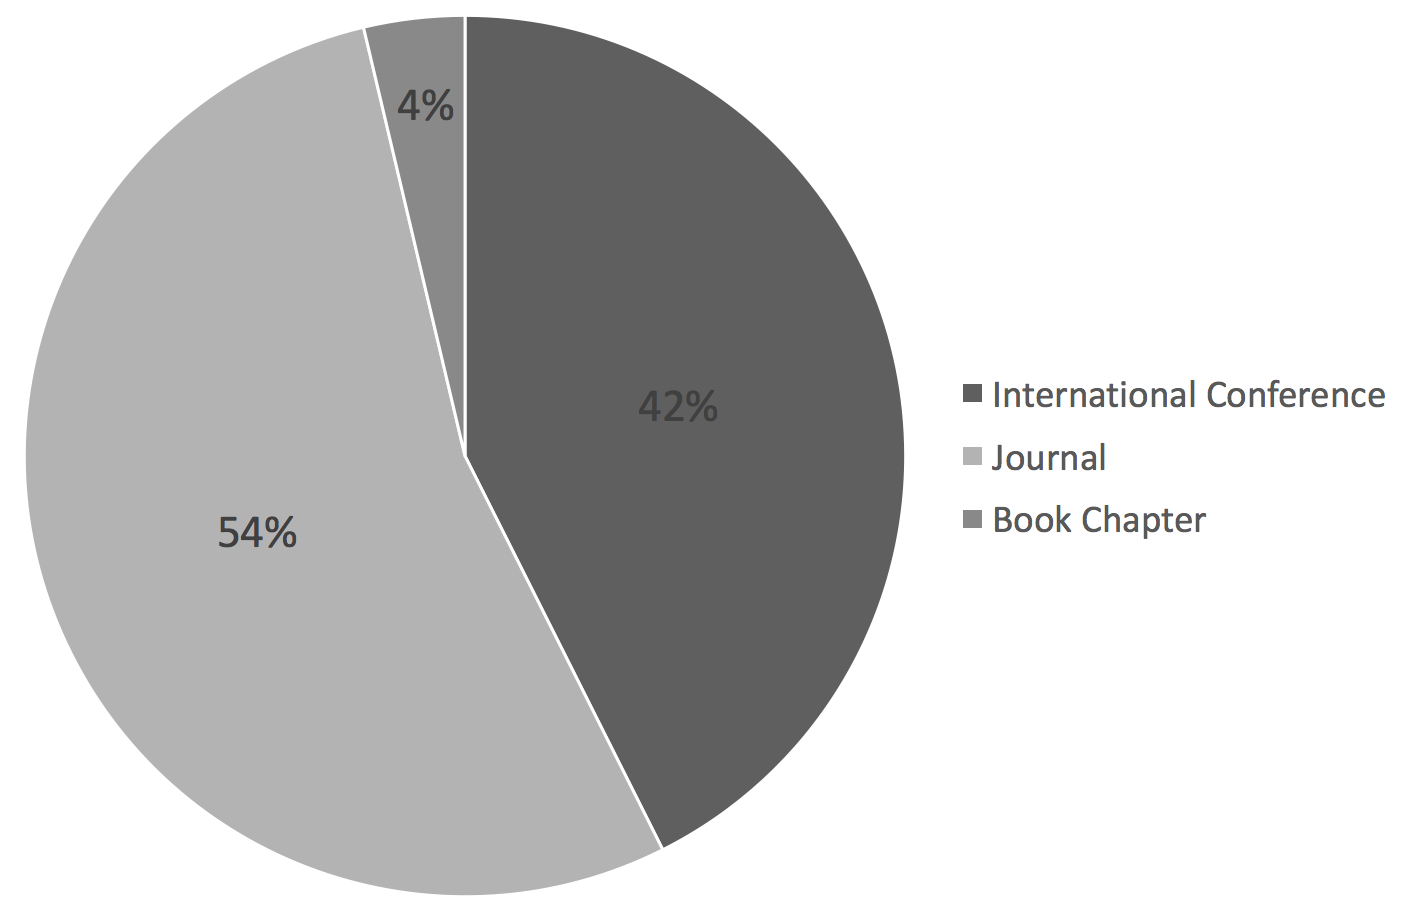
\includegraphics[width=9cm]{img/publication}
% \caption{Types of publication.}
% \label{fig:publications}
% \end{figure}


\subsection*{RQ3: application of technology}

The technological pattern involved in smart-city learning is, most of the times, connected to support the learning process (Fig. \ref{fig:tech_patterns}).
For this purpose, the use of mobile devices is the prevailing choice (Fig. \ref{fig:technology}).
As an example, studies adopt mobile technologies to generate and collect data\cite{philip_framework_2013}\cite{akkerman_storification_2009-1}, support language learning or others school topics and subjects\cite{gaved_challenges_2014} and as supporting technology in situated games in the city\cite{akkerman_storification_2009-1}\cite{huizenga_cognitive_2008}.

\begin{figure}[htb]
\centering
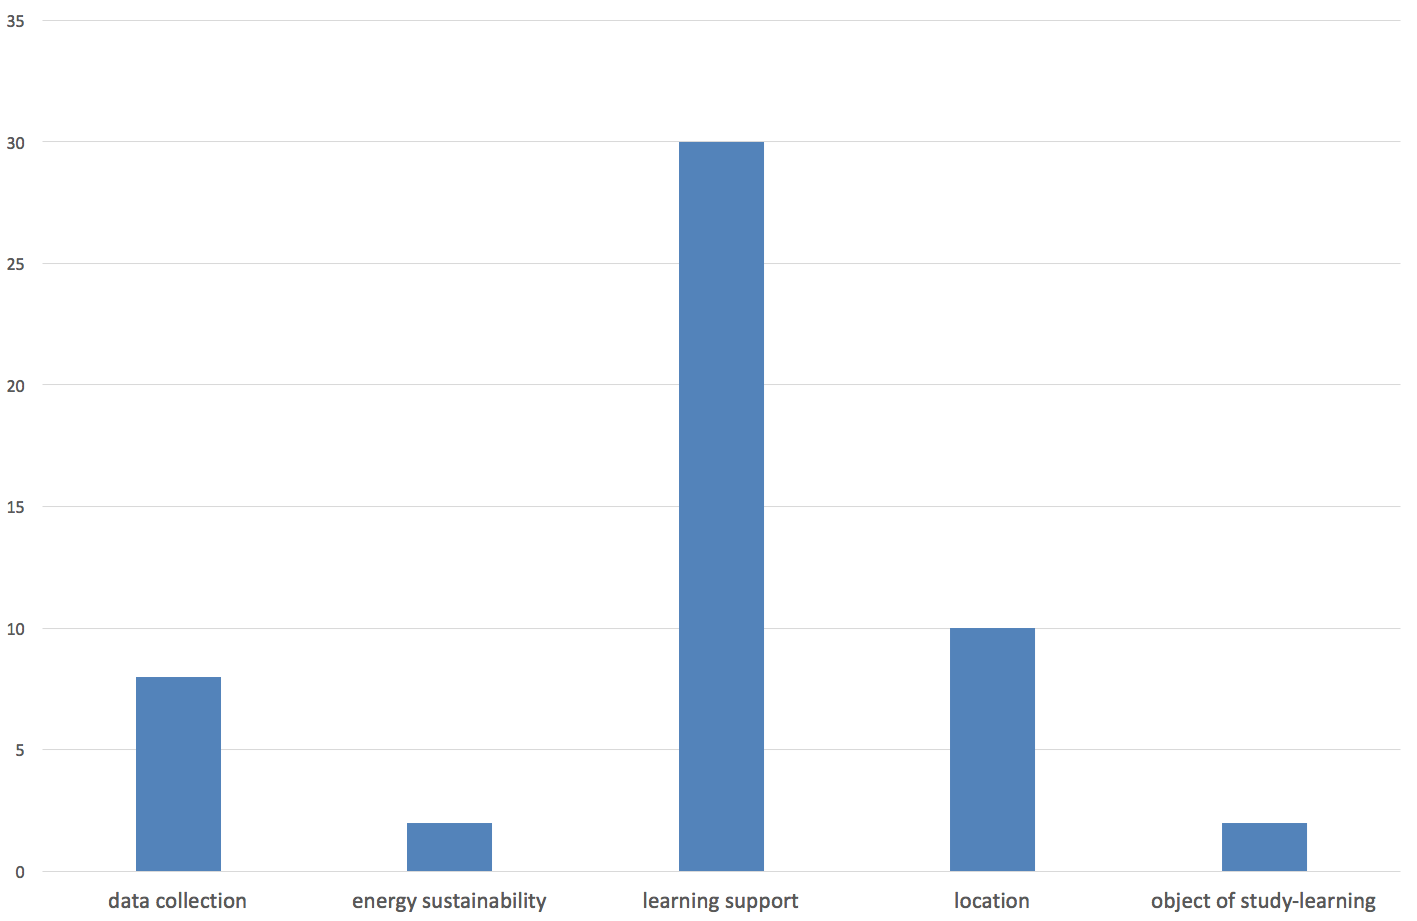
\includegraphics[width=12cm]{img/technological_pattern}
\caption{Identified technological patterns.}
\label{fig:tech_patterns}
\end{figure}

Online cooperative platforms of various types are also used in many cases: more precisely e-learning\cite{schneider_location_2007}\cite{kabaka_elearning_2013} and e-government\cite{wong_prototype_2005}\cite{deakin_intelligent_2012} solutions were mentioned in more than one article.

\begin{figure}[htb]
\centering
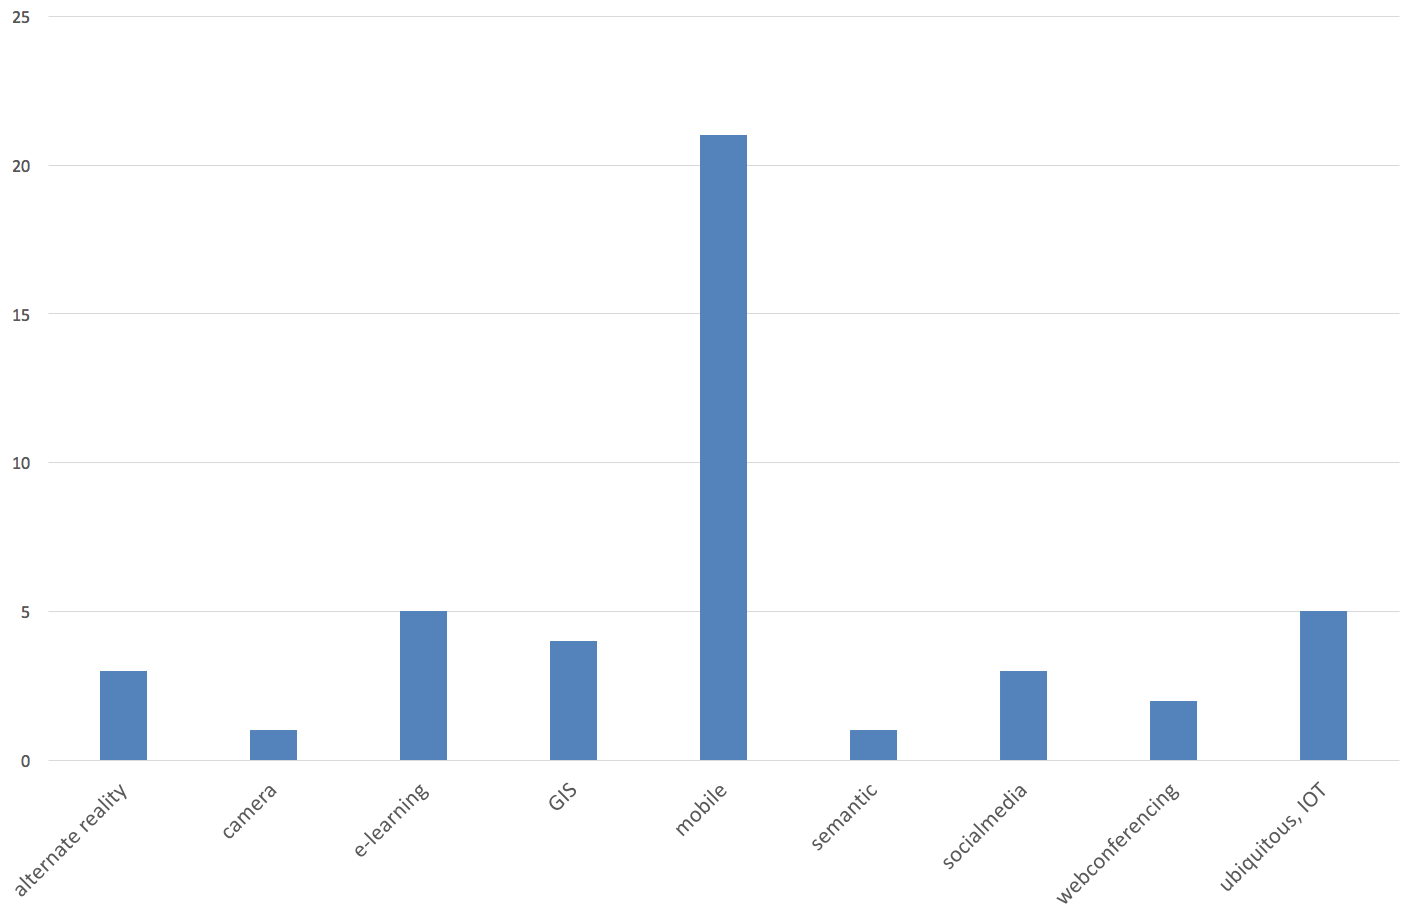
\includegraphics[width=12cm]{img/technology}
\caption{Technology use.}
\label{fig:technology}
\end{figure}


\subsection*{RQ4: learning theories and approaches}

Some articles mentioned specific learning theories applied during the study. Game-based Learning and Situated Learning\cite{anderson_situated_1996} are the approaches that were reported more often (Fig. \ref{fig:learn_theories}).
The articles that follow a Game-Based Learning method usually empower serious games\cite{poplin_digital_2014-2}, the game is often located in the urban space and make use of mobile devices\cite{huizenga_cognitive_2008}.

\begin{figure}[htb]
\centering
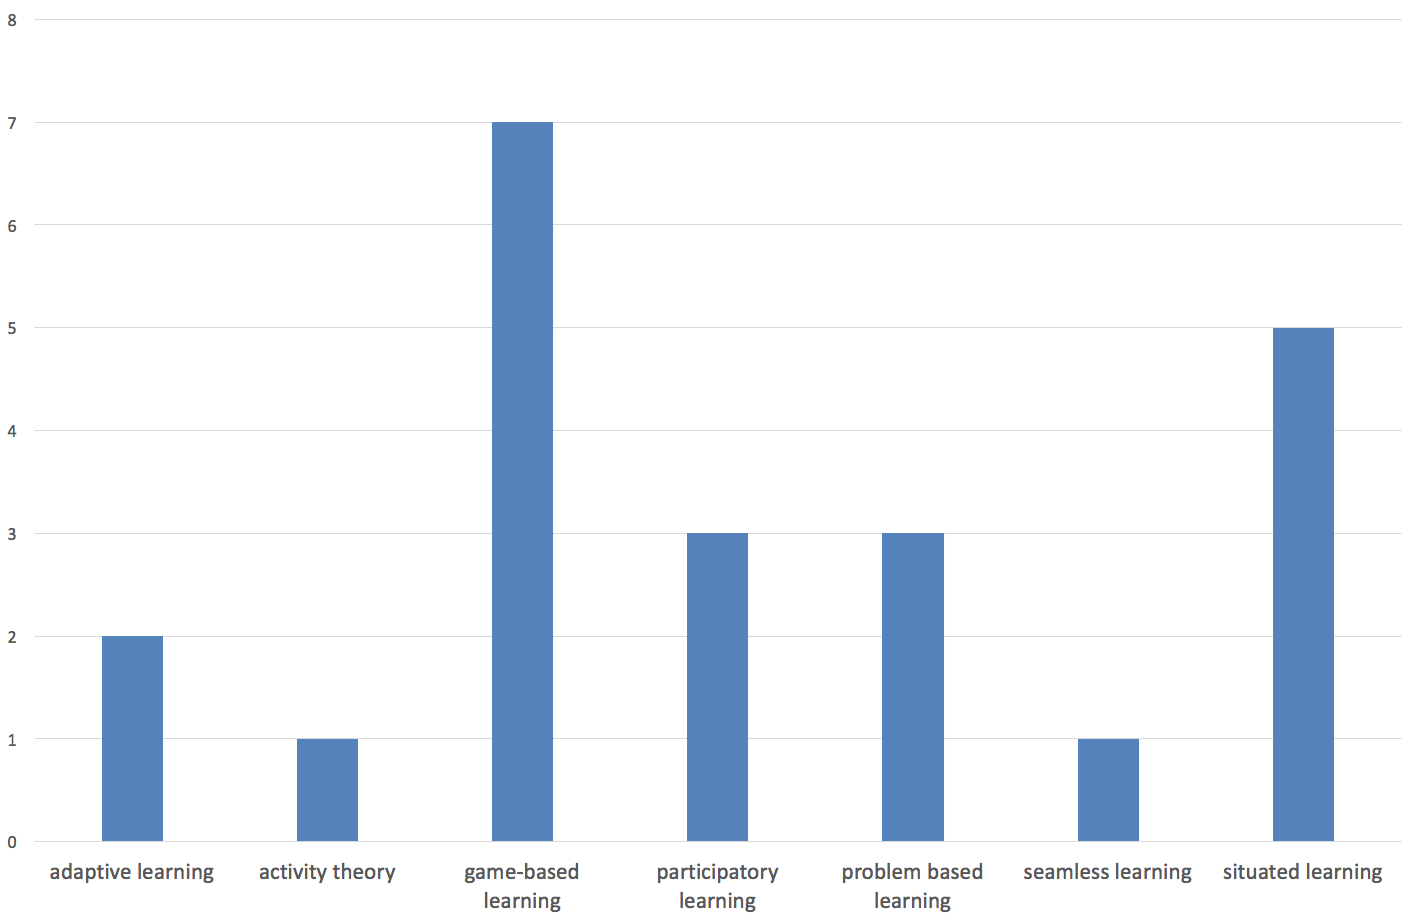
\includegraphics[width=12cm]{img/learning_theories}
\caption{Learning theories applied in the studies.}
\label{fig:learn_theories}
\end{figure}

The approaches that are most often pursued are connected to various levels of collaboration and cooperation between stakeholders or within the learning community (for example among the students). Context awareness and situatedness are also mentioned in a few articles (Fig. \ref{fig:approaches}).

Collaboration is crucial since many articles involves different stakeholders in the learning process, like universities and technical schools\cite{lee_platform_2011}, decision maker, citizens and universities\cite{evans_give_2014} or stakeholders located in different countries\cite{ross_facilitating_2009}\cite{severengiz_enhancing_2015}.

\begin{figure}[htb]
\centering
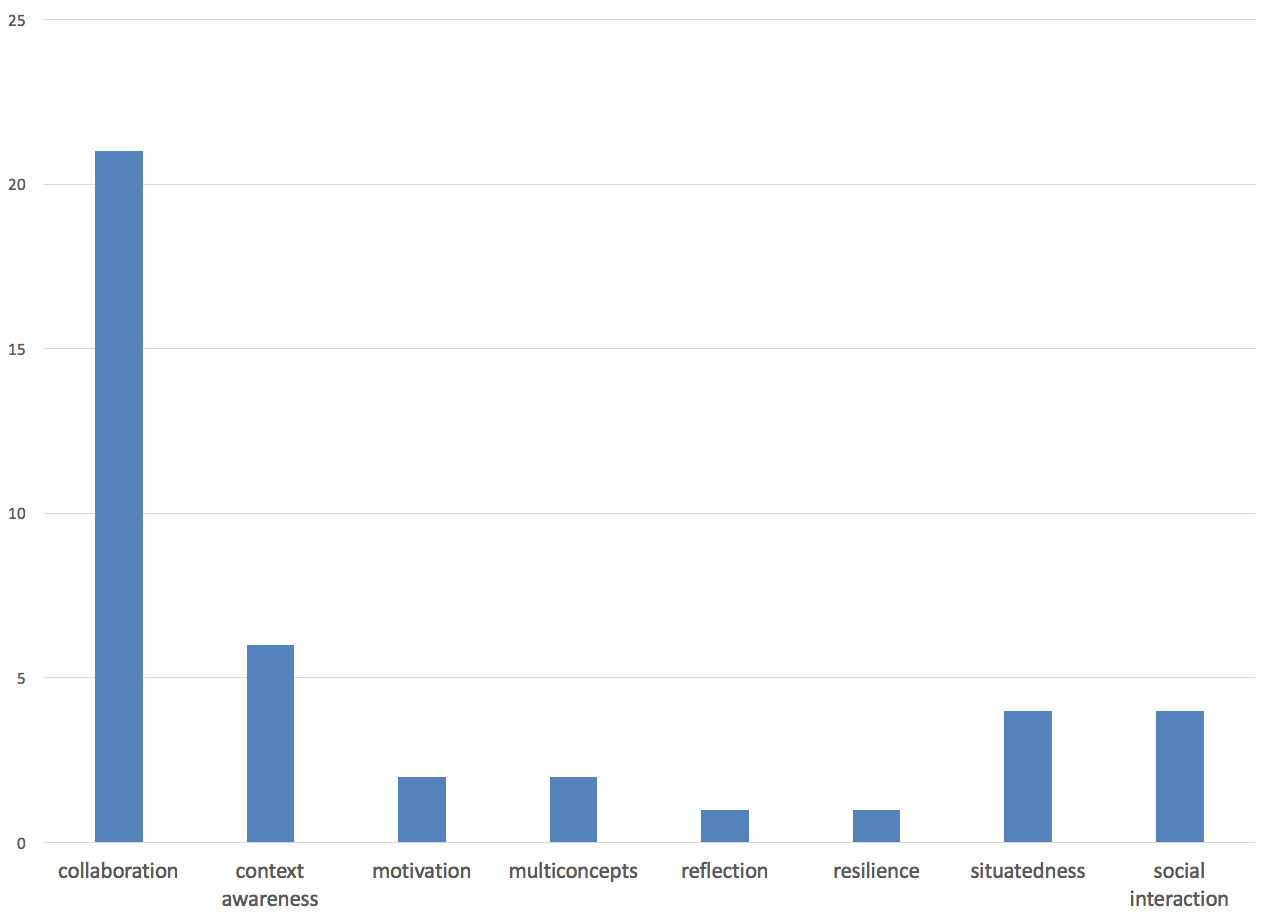
\includegraphics[width=12cm]{img/approaches}
\caption{Pursued approaches and concepts.}
\label{fig:approaches}
\end{figure}


\subsection*{RQ5: research methods and types}
Research on smart-city learning often involves case studies oriented to perform some sort of investigation on a specific problem. Solution design or implementation studies are less common, even more rare are studies that make use of IOT, ubiquitous technologies and custom hardware prototyping.